\documentclass[]{standalone}
\usepackage{tikz}
\usetikzlibrary{chains,fit,shapes}
\begin{document}
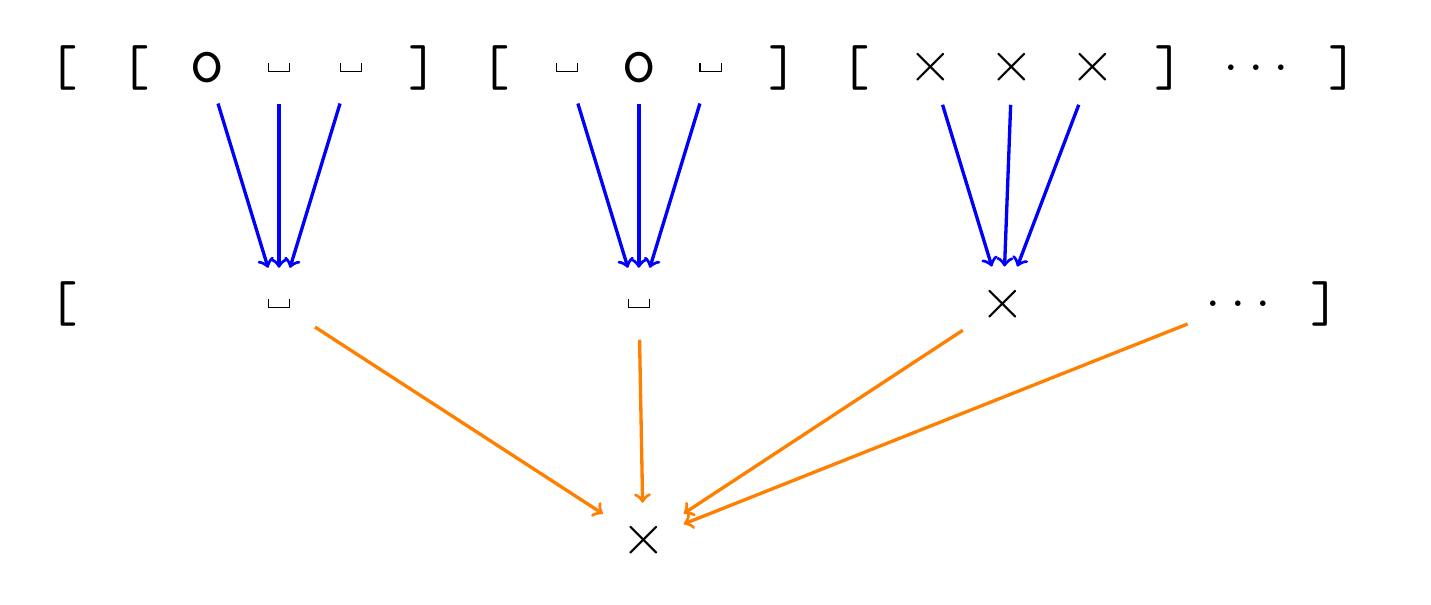
\begin{tikzpicture}
% \tikzstyle{every path}=[thick]

\edef\sizetape{0.9cm}
\tikzstyle{tmtape}=[draw,minimum size=\sizetape]
\tikzstyle{tmhead}=[arrow box,draw,minimum size=.5cm,arrow box
arrows={east:.25cm, west:0.25cm}]

\newcommand\vartextvisiblespace[1][.5em]{%
  \makebox[#1]{%
    \kern.07em
    \vrule height.3ex
    \hrulefill
    \vrule height.3ex
    \kern.07em
  }% <-- don't forget this one!
}

\newcommand{\bola}{\Huge\texttt{o}}
\newcommand{\vazio}{\Huge\vartextvisiblespace}

\fontsize{21}{12}\selectfont

%% Draw TM tape
\begin{scope}[start chain=1 going right,node distance=0mm, draw=none]
    \node [on chain=1,tmtape, draw=none] {\texttt{[}};
    \node [on chain=1,tmtape, draw=none] {\texttt{[}};
    \node [on chain=1,tmtape, draw=none] (c0) {\bola};
    \node [on chain=1,tmtape, draw=none] (c1) {\vazio};
    \node [on chain=1,tmtape, draw=none] (c2) {\vazio};
    \node [on chain=1,tmtape, draw=none] {\texttt{]}};
    \node [on chain=1,tmtape, draw=none] {\texttt{[}};
    \node [on chain=1,tmtape, draw=none] (c3) {\vazio};
    \node [on chain=1,tmtape, draw=none] (c4) {\bola};
    \node [on chain=1,tmtape, draw=none] (c5) {\vazio};
    \node [on chain=1,tmtape, draw=none] {\texttt{]}};
    \node [on chain=1,tmtape, draw=none] {\texttt{[}};
    \node [on chain=1,tmtape, draw=none] (c6) {${\times}$};
    \node [on chain=1,tmtape, draw=none] (c7) {${\times}$};
    \node [on chain=1,tmtape, draw=none] (c8) {${\times}$};
    \node [on chain=1,tmtape, draw=none] {\texttt{]}};
    \node [on chain=1,tmtape, draw=none] {$\ldots$};
    \node [on chain=1,tmtape, draw=none] {\texttt{]}};
\end{scope}

\begin{scope}[shift={(0cm,-3cm)}, start chain=1 going right,node distance=0mm, draw=none]
    \node [on chain=1,tmtape, draw=none] {\texttt{[}};
    \node [on chain=1,tmtape, draw=none] {\texttt{}};
    \node [on chain=1,tmtape, draw=none] {};
    \node [on chain=1,tmtape, draw=none] (w0) {\vazio};
    \node [on chain=1,tmtape, draw=none] {};
    \node [on chain=1,tmtape, draw=none] {\texttt{}};
    \node [on chain=1,tmtape, draw=none] {\texttt{}};
    \node [on chain=1,tmtape, draw=none] {};
    \node [on chain=1,tmtape, draw=none] (w1) {\vazio};
    \node [on chain=1,tmtape, draw=none] {};
    \node [on chain=1,tmtape, draw=none] {};
    \node [on chain=1,tmtape, draw=none] {};
    \node [on chain=1,tmtape, draw=none] {};
    \node [on chain=1,tmtape, draw=none] (w2) {${\times}$};
    \node [on chain=1,tmtape, draw=none] {};
    \node [on chain=1,tmtape, draw=none] {};
    \node [on chain=1,tmtape, draw=none] (rest) {$\ldots$};
    \node [on chain=1,tmtape, draw=none] {\texttt{]}};
\end{scope}

\begin{scope}[shift={(0cm,-6cm)}, start chain=1 going right,node distance=0mm, draw=none]
    \node [on chain=1,tmtape, draw=none] {};
    \node [on chain=1,tmtape, draw=none] {};
    \node [on chain=1,tmtape, draw=none] {};
    \node [on chain=1,tmtape, draw=none] {};
    \node [on chain=1,tmtape, draw=none] {};
    \node [on chain=1,tmtape, draw=none] {};
    \node [on chain=1,tmtape, draw=none] {};
    \node [on chain=1,tmtape, draw=none] {};
    \node [on chain=1,tmtape, draw=none] (wf) {${\times}$};
    \node [on chain=1,tmtape, draw=none] {};
    \node [on chain=1,tmtape, draw=none] {};
    \node [on chain=1,tmtape, draw=none] {};
    \node [on chain=1,tmtape, draw=none] {};
    \node [on chain=1,tmtape, draw=none] {};
    \node [on chain=1,tmtape, draw=none] {};
    \node [on chain=1,tmtape, draw=none] {};
    \node [on chain=1,tmtape, draw=none] {};
    \node [on chain=1,tmtape, draw=none] {};
    \node [on chain=1,tmtape, draw=none] {};
\end{scope}

\draw[->, very thick, blue] (c0) -- (w0);
\draw[->, very thick, blue] (c1) -- (w0);
\draw[->, very thick, blue] (c2) -- (w0);
\draw[->, very thick, blue] (c3) -- (w1);
\draw[->, very thick, blue] (c4) -- (w1);
\draw[->, very thick, blue] (c5) -- (w1);
\draw[->, very thick, blue] (c6) -- (w2);
\draw[->, very thick, blue] (c7) -- (w2);
\draw[->, very thick, blue] (c8) -- (w2);
\draw[->, very thick, orange] (w0) -- (wf);
\draw[->, very thick, orange] (w1) -- (wf);
\draw[->, very thick, orange] (w2) -- (wf);
\draw[->, very thick, orange] (rest) -- (wf);

% %% Draw TM Finite Control
% \begin{scope}
% [shift={(3cm,-5cm)},start chain=circle placed {at=(-\tikzchaincount*60:1.5)}]
% \foreach \i in {q_0,q_1,q_2,q_3,\ddots,q_n}
% 	\node [on chain] {$\i$};

% % Arrow to current state
% \node (center) {};
% \draw[->, very thick] (center) -- (circle-2);

% \node[rounded corners,draw=black,thick,fit=(circle-1) (circle-2) (circle-3) 
%       (circle-4) (circle-5) (circle-6),
% 			label=below:\textbf{Finite Control}] (fsbox)
% 		{};
% \end{scope}

% %% Draw TM head below (input) tape cell
% \node [tmhead,yshift=-.3cm] at (input.south) (head) {$q_1$};

% %% Link Finite Control with Head
% \path[->,draw] (fsbox.north) .. controls (4.5,-1) and (0,-2) .. node[right] 
% 			(headlinetext)
%  			{} 
% 			(head.south);
% \node[xshift=3cm] at (headlinetext)  
% 			{\begin{tabular}{c} 
% 				\textbf{Reading and Writing Head} \\  
% 				\textbf{(moves in both directions)} 
% 			 \end{tabular}};

\end{tikzpicture}
\end{document}